% This document is licensed, at your option, under these or any newer versions of these licenses:
% Creative Commons Attribution 3.0 Unported License
% Creative Commons Attribution 4.0 International License
%
% You should have received a copy of the license along with this work. If not, see:
% <http://creativecommons.org/licenses/by/3.0/>
% <http://creativecommons.org/licenses/by/4.0/>

\documentclass{isprs}
\usepackage{subfigure}
\usepackage{setspace}
\usepackage{geometry} % added 27-02-2014 Markus Englich
\usepackage{epstopdf}
\usepackage{url}
\usepackage[dvipsnames]{xcolor}
\usepackage[colorlinks, allcolors=Blue]{hyperref}
%\usepackage[pdfborderstyle={/S/U/W 1}, citebordercolor=purple, urlbordercolor=blue]{hyperref}
%\usepackage{natbib}

\geometry{a4paper, top=25mm, left=20mm, right=20mm, bottom=25mm, headsep=10mm, footskip=12mm} % added 27-02-2014 Markus Englich
%\usepackage{enumitem}

%\usepackage{isprs}
%\usepackage[perpage,para,symbol*]{footmisc}

%\renewcommand*{\thefootnote}{\fnsymbol{footnote}}



\begin{document}

\title{VALIDATION STRATEGY COMPARISON FOR PLS REGRESSIONS}

\author{
 D. Masili\=unas\textsuperscript{a}}

\address
{
	\textsuperscript{a }Wageningen University, Droevendaalsesteeg 3, NL 6708 PB, Wageningen, The Netherlands - dainius.masiliunas@wur.nl
}

\icwg{}   %This field is NOT optional after all.

\abstract
{
Cross-validation and holdout validation are important tools for the assessment of model accuracy and play an important role in the calibration of Partial Least Squares regression models. We test various cross-validation (Leave-one-out, random, interleaved and consecutive) and holdout validation (simple random, stratified random, bootstrapping, Kennard-Stone and OptiSim) sampling methods using two hyperspectral soil reflectance datasets. Results show little difference between tested cross-validation methods, aside from consecutive sampling that performs worse. All cross-validation methods suggest using a very high number of latent variables for model calibration, which causes the model to have low external prediction power. For holdout validation, Kennard-Stone sampling consistently performs the best. However, it performs better with a low number of samples in the training set when used for external prediction, and with a high number of samples when used for internal prediction. Other sampling methods tested perform similarly to each other, when Monte Carlo simulation is applied to the random sampling methods. Bootstrap sampling gives slightly higher RMSE values than other random sampling methods, whereas OptiSim performs better than other methods only in specific cases. We suggest using Kennard-Stone sampling to calibrate the training set, with a 1:1 split between training and validation sets if external validation is not available, and a 1:2 split if external prediction is a goal of the model.
}

\keywords{PLSR, cross-validation, sampling, soil, spectroscopy}

\maketitle

\section{INTRODUCTION}\label{INTRODUCTION}

Validation is an important step in the creation process of statistical models used for prediction, as it determines how well the model performs in practice and whether it is reliable enough for the required use-case. Validation also gives insight into how many samples of the population need to be taken to achieve a certain model accuracy level. There is a number of different validation methods, and they may have a different effect depending on the model used. In this paper we look at the validation strategies for use with Partial Least Squares Regression (PLSR) models applied to hyperspectral soil reflectance datasets.

Two types of model validation are important in PLSR models: holdout (true, conventional) validation and cross-validation. In holdout validation, the total sample set is divided into two subsets: a training (model building) and validation (test) sets. Only the training set is used for calibrating the model. In other words, the model is optimised in a way that the predictor best fits all samples in the training set. The validation set is put aside, in order to more realistically assess the model performance after it has already been calibrated \cite{kohavi1995study}. The drawback to holdout validation is that by holding back some of the samples, the sample size to which a model is calibrated becomes smaller, and thus the model accuracy suffers. In order to achieve the same level of accuracy as when not doing holdout validation, extra samples equal to the validation set size need to be collected, which can be a costly and time-consuming task.

In contrast, in cross-validation, all available samples in the model are used for both calibration and validation. The validation step is made possible by temporarily splitting the full sample set into training and validation sets, as in holdout validation, but it is repeated a number of times with different ways of splitting, so that every sample goes in both the training and validation set at least once. Then a summary statistic is calculated and used to determine the model accuracy \cite{kohavi1995study}. The drawback to cross-validation is that since all samples are used in the model, it cannot be utilised as a way to optimise the model for better external validity by dropping samples without worthwhile information from the training set. In addition, cross-validation tends to produce overly optimistic results, since the model takes the samples used for validation into account \cite{clark2003boosted}.

There are numerous strategies for splitting the samples into training and validation sets for each of the validation types. There have been studies comparing some cross-validation strategies for hyperspectral data \cite{molinaro2005prediction}, as well as holdout validation strategies \cite{roy2008exploring}, also for PLSR models \cite{clark2003boosted}, but to date there has not been a comprehensive study comparing both holdout and cross-validation methods when applied to the hyperspectral PLSR models used specifically in earth observation. In this paper, we take a look at how using different cross-validation techniques influences the selection of the optimal number of components to use for model calibration, and how model accuracy scales with sample size when different holdout validation techniques are used, when a hyperspectral soil reflectance dataset is used for the PLSR model.

\section{MATERIAL AND METHODS}\label{sec:METHODS}

\subsection{Data}\label{sec:Data}

The models used for this paper were created by using the Netherlands soil spectra dataset made by Alterra \cite{groenestijn2009}. Samples in the dataset (297 in total) were taken by imaging a variety of soil samples using a field spectrometer, after the samples were dried and sieved. The spectral resolution of the spectrometer was 1 nm, and the spectral range was from 420 nm to 2500 nm. The samples were taken predominantly from clay soils.

For assessing the external performance of the resulting models, the Australian soil spectra dataset \cite{rossel2010using}, provided in the \textit{R} package \textit{inspectr}, was used as a validation set (100 samples in total). The samples are from a variety of Australian soils, imaged with a spectrometer with 1 nm spectral resolution and 350-2500 nm spectral range.

\subsection{Cross-validation strategies}\label{sec:Cross-validation strategies}

In order to assess how cross-validation techniques influence the selection of the number of components, the \textit{R} package \textit{plsr} was used, specifically the function \textit{validationplot()} with different cross-validation parameters available in the package. Generated validation plots show how the root mean square error of prediction (RMSEP, also called RMSECV or just RMSE) changes with an increasing number of latent vectors used in the regression. Specifically, RMSE values adjusted for the number of degrees of freedom (Adjusted RMSE, or AdjCV) were used.

Tested cross-validation sampling strategies were: Leave-one-out (LOO), random, interleaved and consecutive sampling, as well as the mean of 100 Monte Carlo (MC) runs of random sampling. For sampling strategies other than LOO, the full data set was divided into two subsets validated against each other (2-fold cross-validation). If the number of subsets \textit{k} is increased, the resulting curve gets closer and closer to the curve of LOO cross-validation (see figure \ref{fig:interleaved-group-sizes}), and at 16 groups is already very close to LOO, hence testing more than 2-fold cross-validation would not give much new information.

\begin{figure}[ht!]
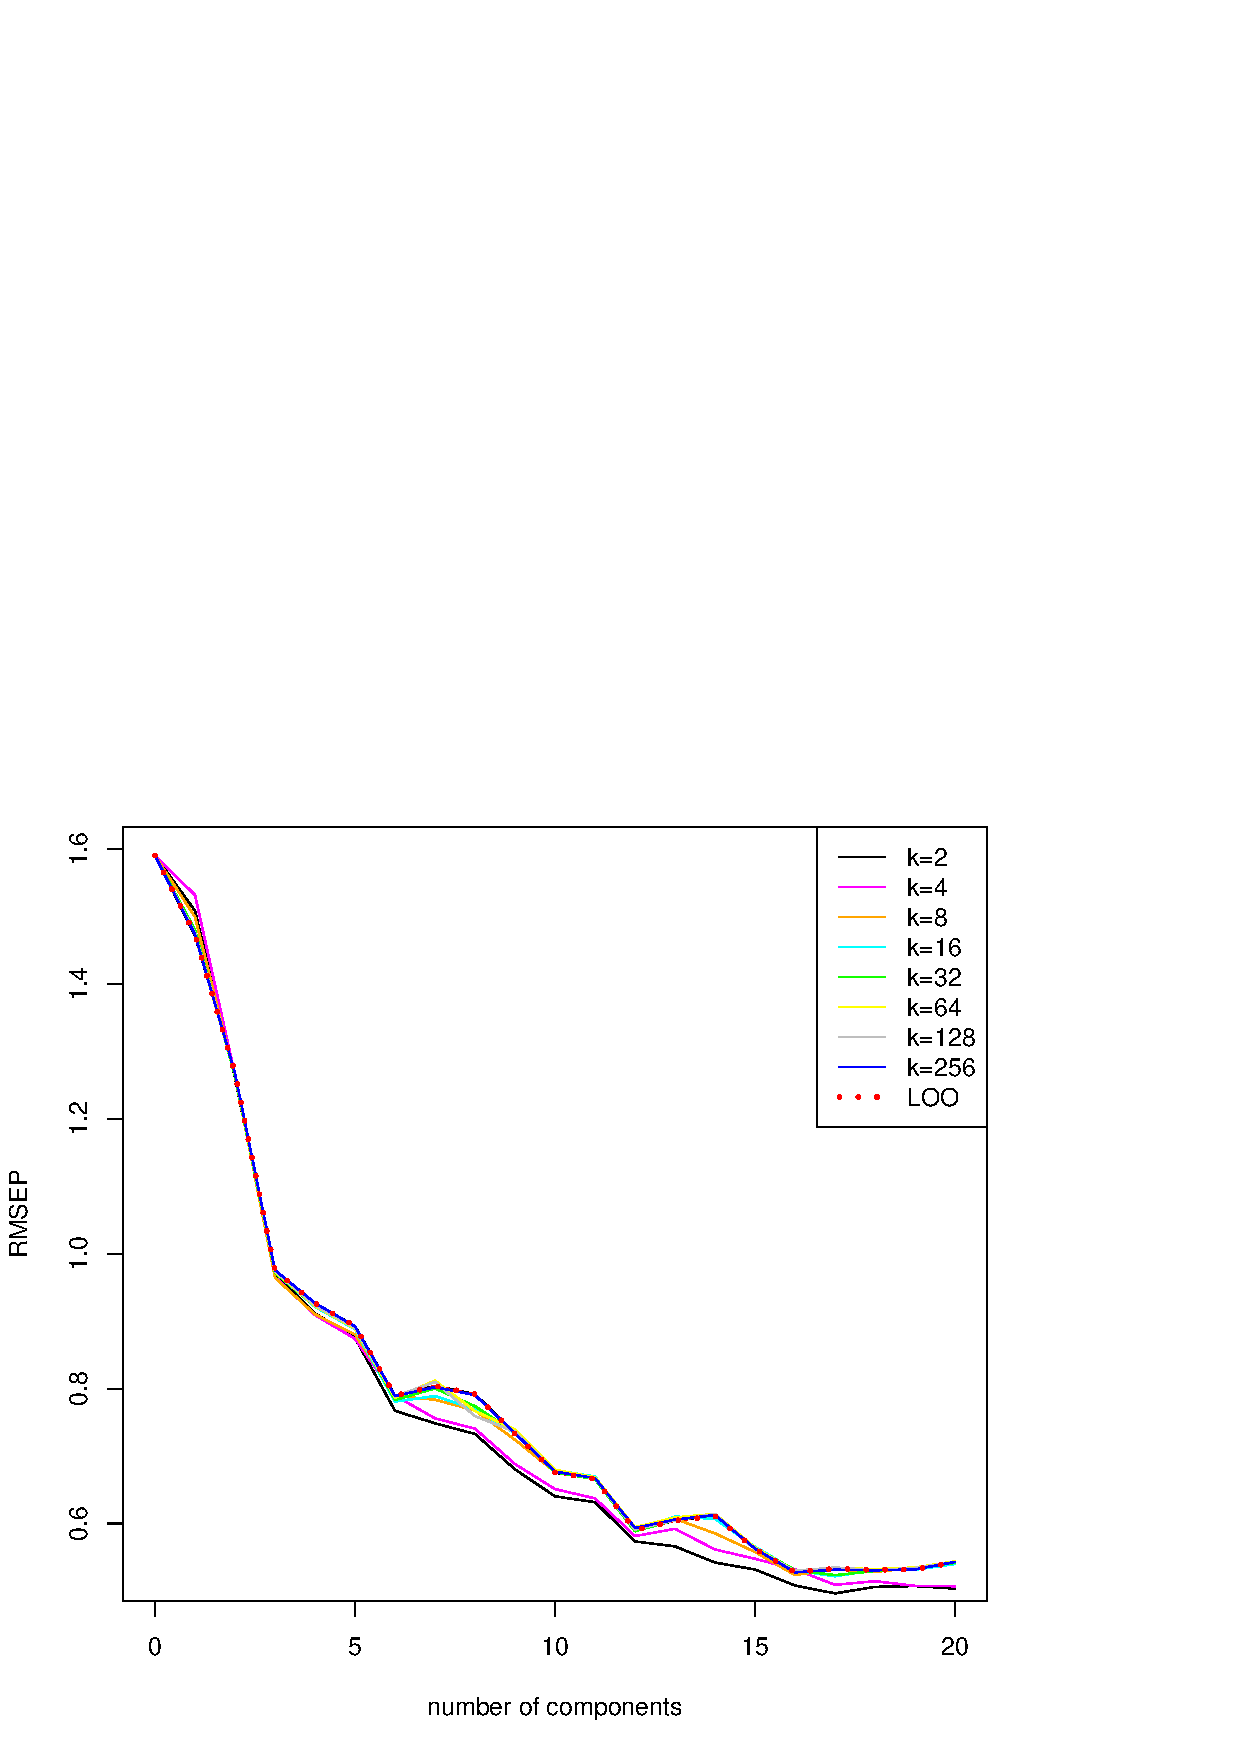
\includegraphics[width=1.0\columnwidth]{../script/output/interleaved-group-sizes.pdf}
\begin{center}
    \caption{Cross-validation plot for model calibration, using interleaved sampling with an increasing number of cross-validation subsets \textit{k}, compared to Leave-one-out validation. The model used all samples from the Netherlands soil spectra dataset. Lower root mean square error of prediction (RMSEP) values per latent vector (component) number used by the model indicate a better model fit for the input samples.}
    \label{fig:interleaved-group-sizes}
\end{center}
\end{figure}

\subsection{Holdout validation strategies}\label{sec:Holdout validation strategies}

For assessing holdout validation techniques, samples were split into training and validation sets manually for random without replacement, random with replacement (bootstrapping) and stratified random sampling. For the respective Monte Carlo simulations, the splitting into different sets was repeated 100 times, and the result was averaged over all runs. In addition, Kennard-Stone and OptiSim sampling was tested. For Kennard-Stone sampling, the \textit{inspectr} package was used to generate the validation sample set, based on the Kennard-Stone maximum difference algorithm \cite{kennard1969computer}. For OptiSim sampling \cite{clark1997optisim}, the latest in-development code from the \textit{inspectr} package was used. The OptiSim algorithm is also a differencing algorithm like Kennard-Stone, but instead of differencing every sample against each other, cluster means are differenced instead. OptiSim sampling was run using clusters of 4 samples (\textit{k} = 4), since studies have shown that this setting generally performs the best on hyperspectral datasets \cite{clark2003boosted}.

Two strata were used for stratified random sampling: one stratum included samples with pH below the median pH for all samples (6.11), and the other included all samples equal or above the median. The strata were chosen as such because pH distribution among samples is bimodal, with fewer values around the median value (which is also close to the neutral pH value of 7). Splitting the strata at the median allows for balanced strata, without the need to use bootstrapping or drop samples.

Validation was repeated twice, once for internal and once for external validation: the first time the validation set used all unused samples from the same Netherlands soil dataset as the training set, whereas the second time the full external Australian soil dataset was used for validation.

In addition, the above analysis was repeated twice, using different numbers of latent vectors for the PLS regression (16 and 6), in order to see how the choice of the number of latent vectors from the model calibration step impacts the PLS regression and the resulting holdout validation scores.

\section{RESULTS}\label{sec:RESULTS}

\subsection{Cross-validation strategies}\label{sec:Cross-validation strategies 2}

The cross-validation sampling strategies for the Netherlands soil dataset used produced similar results to one another, with the overall shape of the RMSE vs latent vector number curve being the same across all the tested strategies except for consecutive sampling (see figure \ref{fig:cv}). Consecutive sampling resulted in higher RMSE values than other strategies, yet it still reached the minimum RMSE value (0.70) at 16 latent vectors used in the model, just like with the LOO cross-validation strategy (in which case the RMSE was 0.53).

The random sampling strategy results in an unstable minimum RMSE value, since the full data set is split into two subsets randomly. Running Monte Carlo analysis of random sampling gives more stable results (depending on the number of runs) which are also closer to those obtained by LOO cross-validation. The Monte Carlo standard deviation (mean of standard deviations at each number of latent vectors) was 0.02.

Of all the cross-validation strategies tested, the lowest RMSE values were obtained using interleaved cross-validation (see figure \ref{fig:cv}), however, whether interleaved cross-validation is suitable for use depends on the way the dataset is laid out. Monte Carlo simulation of random sampling resulted in the second lowest RMSE values, and LOO cross-validation had third lowest RMSE values.

The absolute minimum RMSE was obtained using 16 (consecutive, LOO) or 17 (interleaved, Monte Carlo) latent vectors, and had similar values in the 16-20 latent vector range. Therefore holdout validation analysis was first done using 16 latent vectors. Then it was repeated using 6 latent vectors, since it is the first local RMSE minimum for both LOO and consecutive cross-validation results.

\begin{figure}[ht!]
\includegraphics[width=1.0\columnwidth]{../script/output/cv.pdf}
\begin{center}
    \caption{PLSR cross-validation plot for calibration, when using different sampling strategies. The model used all samples from the Netherlands soil spectra dataset.}
    \label{fig:cv}
\end{center}
\end{figure}

\subsection{Holdout validation strategies}\label{sec:Holdout validation strategies 2}

\subsubsection{Netherlands soil validation, 16 latent vectors:}\label{sec:NL16}

When comparing how RMSE values change as the number of samples used in the PLS regression increases using various holdout validation strategies, with validation samples from the same dataset, we can see a typical pattern of RMSE gradually going down until it becomes stable at around 150 samples for most sampling strategies (see figure \ref{fig:rmse-nl-16}).

Just like with cross-validation, sampling methods that have a random component to them (simple and stratified random sampling as well as bootstrapping) are not consistent when performed only once and require Monte Carlo simulations to reduce the variance of results. The Monte Carlo standard deviation of these methods is generally higher towards the edges, that is, when either the training or the validation set sizes become low.

Stratified and simple random sampling after 100 Monte Carlo runs result in very similar RMSE values, whereas bootstrapping gives slightly higher RMSE values.

Kennard-Stone sampling results in the lowest RMSE values, no matter the sample size. OptiSim sampling performs very poorly when the training set size is very low, but quickly gets better as more samples are added to the training set. It even overtook Kennard-Stone sampling at 56 samples in the training set, however, OptiSim also involves a random component, so repeated runs might give slightly different results. When the training set size is increased over 56 samples, RMSE values of OptiSim are no longer any lower than when using simple or stratified Monte Carlo methods.

The ratio of standard deviation of the training set to RMSE (RPD) values exceeded 3 for Kennard-Stone sampling starting from 132 samples in the training set (with a maximum of 3.58 RPD at 240 samples), and never for the other sampling methods (not counting random-based sampling without Monte Carlo), although at the maximum of 256 samples, Monte Carlo simple random sampling achieved an RPD of 2.98.

\begin{figure}[ht!]
\includegraphics[width=1.0\columnwidth]{../script/output/rmse-nl-16.pdf}
\begin{center}
    \caption{Performance of various holdout validation strategies as the training set size increases. The validation set consists of all samples from the Netherlands soil dataset not used in the training set, number of latent vectors used is 16.}
    \label{fig:rmse-nl-16}
\end{center}
\end{figure}

\subsubsection{Australian soil validation, 16 latent vectors:}\label{sec:AU16}

The results when using an independent validation set are completely different (see figure \ref{fig:rmse-au-16}). Most sampling strategies produce a flat line for RMSE, meaning that adding more samples into the model has no effect at all on the pH prediction accuracy in Australian soils, when the model is calibrated for Netherlands soil data.

Kennard-Stone sampling, when the training set is small (less than 100 samples), consistently performs better than random sampling methods, but as the training set increases, it is no longer distinguishable from the random sampling methods.

RPD values never exceeded 0.4 even when the single runs of random sampling methods are taken into account. Thus while the internal prediction of the model when using random Monte Carlo and Kennard-Stone sampling is good enough for screening, the external predictive power of the same model is extremely poor.

\begin{figure}[ht!]
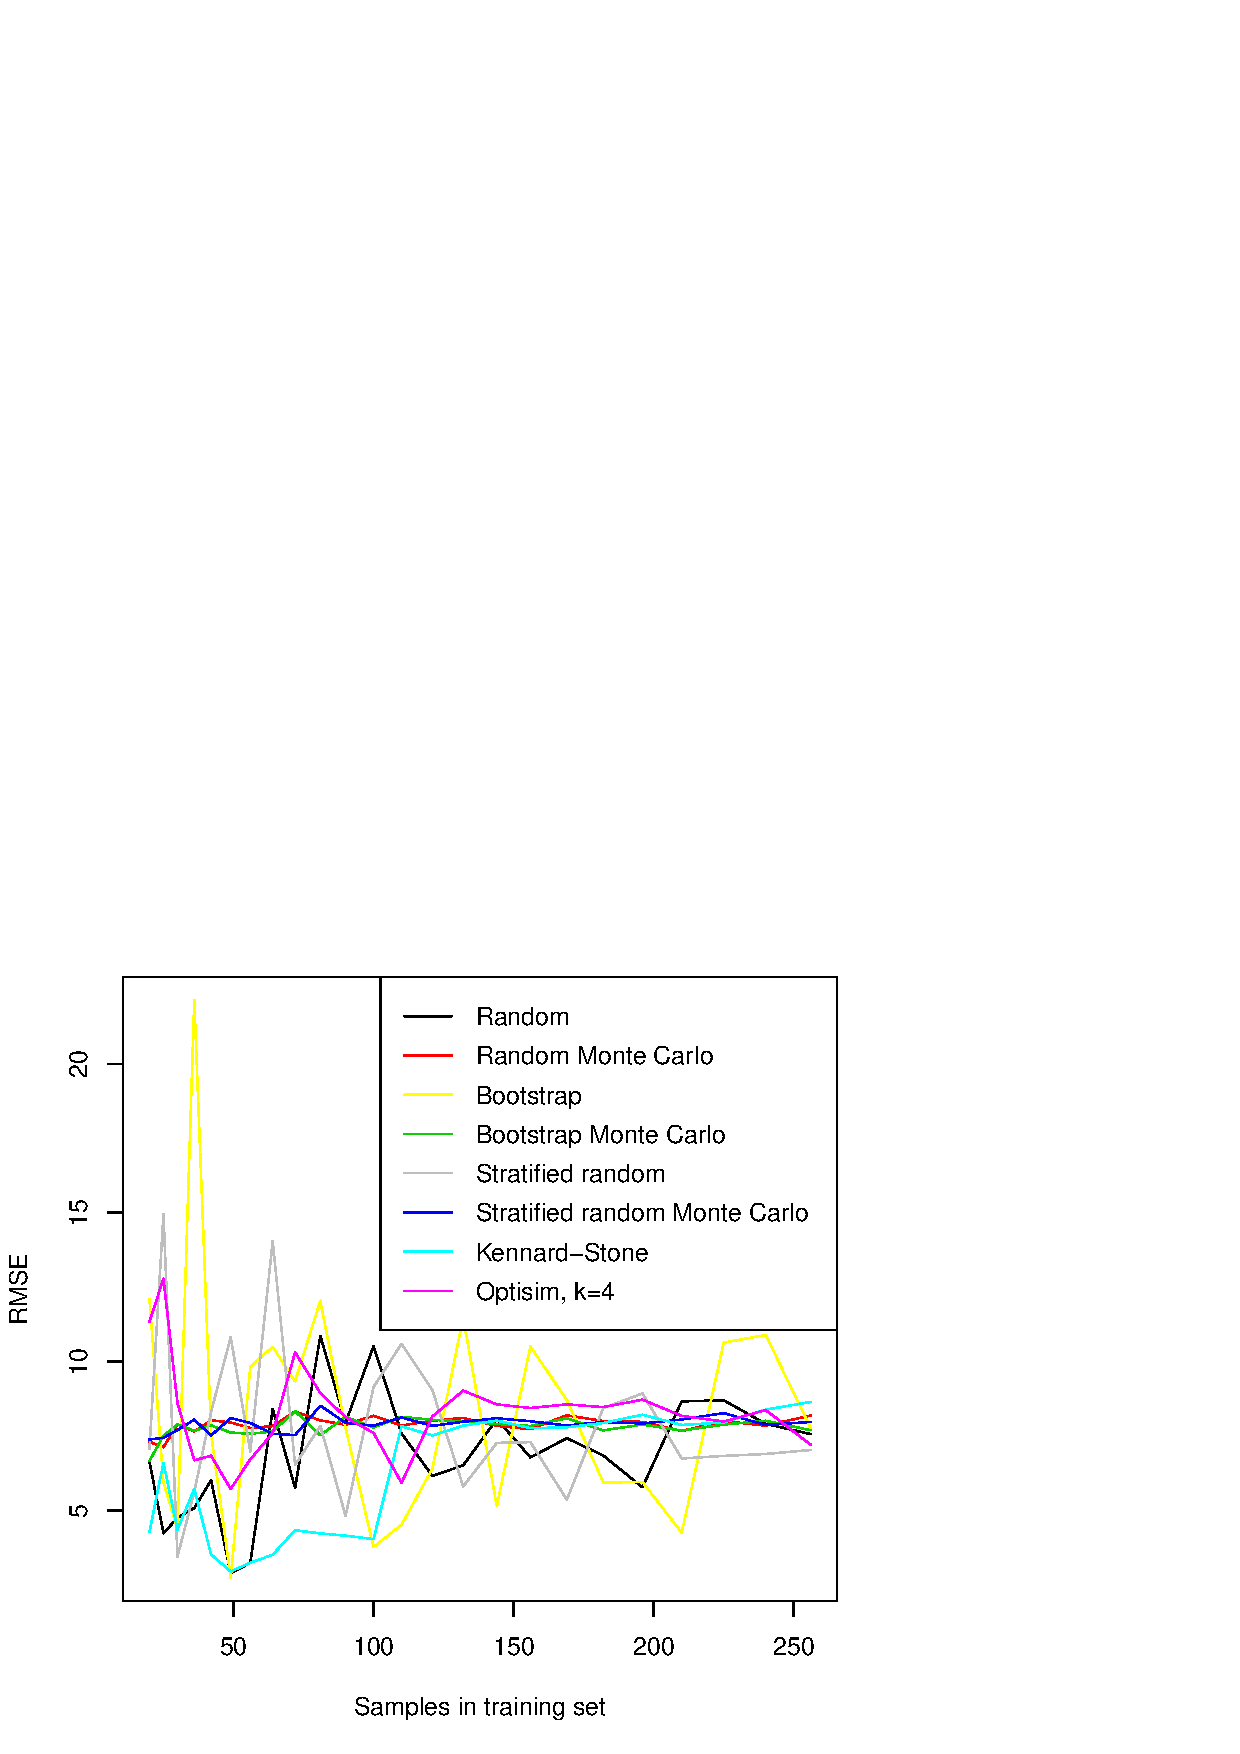
\includegraphics[width=1.0\columnwidth]{../script/output/rmse-au-16.pdf}
\begin{center}
    \caption{Performance of various holdout validation strategies as the training set size increases. The validation set consists of all samples in the Australian soil dataset, number of latent vectors used is 16.}
    \label{fig:rmse-au-16}
\end{center}
\end{figure}

\subsubsection{Netherlands soil validation, 6 latent vectors:}\label{sec:NL6}

When the analysis is repeated for a model using 6 latent vectors, using the Netherlands data for validation, the general pattern stays the same as for 16 latent vectors (see figure \ref{fig:rmse-nl-6}). The main differences are the RMSE values, which are higher (as already shown in the calibration phase), and the patterns for Kennard-Stone sampling as well as OptiSim.

At a low number of samples in the training set, Kennard-Stone sampling performs worse than any other sampling method (not counting single random realisations), but evens out at 125 training set samples and has lower RMSE values than other sampling methods as the number of training samples increases past 150. The pattern for OptiSim sampling is contrary to that of Kennard-Stone, with OptiSim performing the best when the training set is small and worse than the random methods when the training set is larger than 150 samples.

As expected, none of the sampling methods ever achieve an RPD close to 3 when using only 6 latent vectors, with the maximum achieved by Kennard-Stone sampling at 2.12.

\begin{figure}[ht!]
\includegraphics[width=1.0\columnwidth]{../script/output/rmse-nl-6.pdf}
\begin{center}
    \caption{Performance of various holdout validation strategies as the training set size increases. The validation set consists of all samples from the same dataset not used in the training set, number of latent vectors used is 6.}
    \label{fig:rmse-nl-6}
\end{center}
\end{figure}

\subsubsection{Australian soil validation, 6 latent vectors:}\label{sec:AU6}

When the Australian dataset is used for validation at 6 latent vectors, there are notable changes from when 16 components were used (see figure \ref{fig:rmse-au-6}). The RMSE values are overall lower. The random sampling methods in this case show a small decrease in RMSE when the training set size is increased up to 50, but flattens out after that.

Kennard-Stone sampling shows an even more pronounced inverse curve than in the 16 latent vector case, with the RMSE increasing as more samples are added into the training set, with lower RMSE values than other sampling methods. On the other hand, OptiSim starts out performing worse than the other sampling methods, but the RMSE value gets progressively closer to that of the random methods. The highest RPD value achieved by Kennard-Stone sampling is 0.89 at only 20 samples in the training set.

\begin{figure}[ht!]
\includegraphics[width=1.0\columnwidth]{../script/output/rmse-au-6.pdf}
\begin{center}
    \caption{Performance of various holdout validation strategies as the training set size increases. The validation set consists of all samples in the Australian soil dataset, number of latent vectors used is 6. The colours represent the same methods as in previous graphs.}
    \label{fig:rmse-au-6}
\end{center}
\end{figure}

\section{DISCUSSION}\label{sec:DISCUSSION}

\subsection{Cross-validation strategies}\label{sec:Cross-validation strategies 3}

From the cross-validation strategies tested, each has its own peculiarities. Random sampling gives results that are not stable, therefore at low \textit{k} it is not suitable for determining the optimal number of latent vectors to use in the regression by itself. However, since for the dataset used the standard deviation of random sampling was low, using Monte Carlo random sampling, even with relatively low number of runs, is an option. Generally it gives results very similar to that of Leave-one-out cross-validation.

Leave-one-out cross-validation result itself is deterministic, however, it requires recalculating the PLS regression for every sample included in the model, thus it takes more time than all other cross-validation strategies tested (aside from Monte Carlo, which can have an arbitrarily high number of runs).

Interleaved sampling in this case gave good results, was fast and deterministic, however, it depends on the way the dataset is organised. Often times datasets are ordered by how the samples were taken, for instance, by starting collecting samples at one end of an area and finishing at the other. However, if every or nearly every other sample was taken from an area with different properties, then the subsets of interleaved samples will no longer be representative of one another and result in unusually high RMSE values. Therefore choosing interleaved sampling with no \textit{a priori} knowledge of how the dataset was made is risky and may lead to an incorrect choice of latent vectors to use.

That is what happened in this case with consecutive sampling. If there is a gradient or a jump in values in the dataset due to physical properties at one end of an area being different from the other end of it, consecutive sampling will produce subsets that are not representative of one another.

\subsection{Holdout validation strategies}\label{sec:Holdout validation strategies 3}

From the holdout validation strategies tested, Kennard-Stone sampling performed the best in all cases. This is due to the Kennard-Stone algorithm selecting samples of highest difference from the dataset first. Since those samples have the largest variation, they also hold most of the information about the data collected, and the rest of the samples (which are less extreme) are used for validation, thus resulting in a consistently lower RMSE. This is in line with the results of other studies using similar differencing methods on hyperspectral data \cite{golbraikh2000predictive}. However, calculating the differences between each of the samples takes a lot of time and computing power. In addition, if the validation set is derived from the same dataset as the training set, and is too small, the RMSE values become unrealistically low, since the validation set only contains the least different (hence easiest to predict) samples.

OptiSim sampling performed better than other sampling methods only when using Netherlands soil validation with 6 latent vectors, when using small training set sizes. Otherwise it performed equally to or even worse than random sampling methods. This is surprising, compared to other studies, where OptiSim sampling was performing better for external validation and worse for internal validation than random sampling \cite{clark2003boosted}, and indicates that the results may vary depending on the model and type of external validation chosen.

Stratified random sampling generally performed the same as simple random sampling. This is likely to be due to the rather simplistic method of stratifying chosen. If there was any extra data about the soil type that each spectrum represented, and it was used as the stratification criterion, then stratified sampling might have been more distinguishable from simple random sampling, as shown in other studies \cite{kohavi1995study}.

Bootstrap sampling performed worse than random sampling without replacement, since samples were duplicated. This acts opposite of the Kennard-Stone method, with more redundant data going into the training set, and the model overfitting those samples, compared to the remaining ones (that were used for validation).

When the Australian soil dataset was used for validation, the model fit was poor for all sampling methods when using 16 latent vectors in the model, with a maximum RPD of 0.4, in stark contrast with the model fit when the same dataset was used for validation. This indicates that the model is overfitting for the samples in the training dataset, resulting in little to no predictive power outside the training dataset. This is expected, since 16 latent vectors is a very high number for typical applications, and the last latent vectors are likely to not contain any information useful for external prediction at all.

Unfortunately, none of the cross-validation strategies indicated such a problem, with most of them agreeing that 16 latent vectors is the optimal choice. This confirms that cross-validation tends to be overoptimistic \cite{clark2003boosted}. Therefore choosing a lower number of latent vectors than it might appear optimal from cross-validation graphs is important, if external prediction is the goal of the PLSR model. Perhaps using a statistic other than RMSE, such as the Akaike Information Criterion, or using a training set reduced with Kennard-Stone sampling, would be better when optimising the model for external prediction. In this case, some of the cross-validation graphs indicated a small local minimum at 6 latent vectors, thus the analysis was repeated for that number of latent vectors.

With the reduced number of latent vectors, the predictions about the pH level of the Australian soil dataset have become better, but still not nearly good enough for screening, and adding more samples hardly helps increase prediction accuracy. In the case of Kennard-Stone sampling, a seemingly counter-intuitive pattern is seen, where adding more samples to the training set cosistently decreases prediction accuracy. However, this makes sense given that the algorithm supplies the most extreme samples into the training set first. That helps external accuracy, as soils in the external dataset might deviate strongly from the soils in the internal dataset. As the number of training samples increases, more and more samples close to the mean for the Netherlands dataset are added, making the PLSR model more and more optimised for the particular soil types in the Netherlands dataset, resulting in overfitting.

The low external predictive power of the model might have been caused by the difference in soil types between the Netherlands and Australia, as well as the differences in the equipment used to get hyperspectral data and pH values of the various soils.

\section{CONCLUSIONS}\label{sec:CONCLUSIONS}

There was little difference between all tested cross-validation strategies, only consecutive sampling produced notably higher RMSE values (0.70 minimum, as opposed to 0.53 of LOO) per number of latent variables compared to other sampling methods. All of them suggested 16 or 17 latent variables as optimal for the Netherlands soil PLSR model, although external validation shows that it is too many if external prediction is the goal of the model. Thus other methods or statistics should be explored in order to better calibrate such models for external prediction.

From all tested holdout validation strategies, Kennard-Stone sampling performed the best across all tested cases, however, the optimal training set size differed. When samples internal to the dataset were used for validation, increasing the training set size resulted in lower RMSE, but it is the other way round when an external dataset was used as validation. Thus if the model is intended for external prediction, then using a relatively small sample chosen by the Kennard-Stone algorithm for training (100 or fewer samples in the tested case, which is one third of the full dataset) is the best. If the model is intended for internal prediction, then using a relatively large training set is recommended. However, the validation set also has to be large enough to avoid the validation set becoming artificially too predictable. For the Netherlands soil spectra dataset, a reasonable choice is a split into equal parts for training and validation (148 samples each), in which case, at 16 latent variables, RPD is 3.1.

Other holdout validation strategies gave similar results to each other. For simple, stratified and bootstrap random methods, Monte Carlo simulations are needed to lower the variance of the results. Bootstrap sampling consistently gave higher RMSE values than simple and stratified sampling, and the latter two were nearly indistinguishable. Lastly, OptiSim sampling only gave lower RMSE values in a single instance (low training set size at 6 latent variables using internal validation) and otherwise performed worse or as well as simple random sampling.

{%\footnotesize
	\begin{spacing}{0.9}% tune the size by altering the parameter
		\bibliography{AEO-paper}
	\end{spacing}
}

\section*{APPENDIX}\label{APPENDIX}

The \textit{R} code used to carry out the analysis for this paper is available online, at:

\url{https://github.com/GreatEmerald/AEO-validation-paper}

\end{document}
